\documentclass[12pt,a4paper]{article}

\usepackage{fontspec}
\setmainfont{Times New Roman}
\setmonofont{JetBrainsMono Nerd Font Mono}[Scale=0.85]
\newfontfamily\cyrillicfonttt{Times New Roman}[Scale=0.85]

\usepackage{polyglossia}
\setdefaultlanguage{russian}

\usepackage{geometry}
\geometry{top=2cm,bottom=2cm,left=2.5cm,right=2cm}

\usepackage{graphicx}
\usepackage{float}
\usepackage{caption}
\usepackage{subcaption}
\usepackage{hyperref}
\usepackage{listings}
\usepackage{xcolor}
\usepackage{booktabs}
\usepackage{indentfirst}
\usepackage{parskip}

\hypersetup{
    colorlinks=true,
    linkcolor=black,
    urlcolor=blue,
}

\lstset{
    basicstyle=\small\ttfamily,
    breaklines=true,
    frame=single,
    tabsize=4,
    numbers=left,
    numberstyle=\tiny,
    backgroundcolor=\color{gray!5},
    aboveskip=8pt,
    belowskip=8pt,
}

\title{\textbf{SET 9. Домашняя работа} \\ Строки--2. Сортировка. Кодирование}
\author{Коновалов Иван Андреевич}
\date{25 мая 2026 г.}

\begin{document}

\maketitle
\thispagestyle{empty}

\vspace{2cm}
\begin{center}
\textbf{Алгоритмы и структуры данных} \\
2025--2026 учебный год \\
НИУ ВШЭ
\end{center}

\newpage

\tableofcontents
\newpage

% ─── 1. Codeforces submissions ───────────────────────────────────────────────

\section{ID посылок в системе Codeforces}

Ниже приведены идентификаторы успешных посылок по задачам Блока~A в систему Codeforces. Все реализации прошли полное тестирование с максимальным баллом.

\begin{table}[H]
\centering
\begin{tabular}{llll}
\toprule
\textbf{Задача} & \textbf{ID посылки} & \textbf{Описание} & \textbf{Баллы} \\
\midrule
A1m & 375976675 & String Merge Sort (LCP)      & 5/5 \\
A1q & 375976722 & String Quick Sort (ternary)   & 4/4 \\
A1r & 375976757 & MSD Radix Sort (no cutoff)    & 4/4 \\
A1rq & 375976806 & MSD Radix + Quick Sort hybrid & 3/3 \\
\bottomrule
\end{tabular}
\caption{Посылки адаптированных алгоритмов сортировки строк}
\end{table}

Общий балл за реализацию адаптированных алгоритмов: \textbf{16 из 16}.

\section{Ссылка на репозиторий}

Исходный код, результаты эмпирических замеров (CSV) и графики находятся в публичном репозитории:

\begin{center}
\url{https://github.com/festy23/SET-9-string-sort}
\end{center}

В репозитории представлены:
\begin{itemize}
    \item Классы \texttt{StringGenerator} и \texttt{StringSortTester} (C++);
    \item Реализации шести алгоритмов сортировки с подсчётом посимвольных сравнений;
    \item Решения задач Блока~P (Хаффман, LZW-кодирование, LZW-декодирование);
    \item CSV-файлы с эмпирическими данными в директории \texttt{data/};
    \item Графики в директории \texttt{plots/}.
\end{itemize}

% ─── 2. Infrastructure ───────────────────────────────────────────────────────

\section{Инфраструктура экспериментального анализа}

\subsection{StringGenerator}

Класс \texttt{StringGenerator} предназначен для генерации тестовых массивов строк. Основные параметры:

\begin{itemize}
    \item \textbf{Алфавит:} 74 символа — заглавные латинские буквы A--Z (26), строчные a--z (26), цифры 0--9 (10), специальные символы \texttt{!@\#\%:;\^{}\&*()-} (12);
    \item \textbf{Длина строк:} равномерное распределение от 10 до 200 символов;
    \item \textbf{Размеры массивов:} от 100 до 3000 строк с шагом 100 (30 размеров).
\end{itemize}

Для каждого типа данных генерируется мастер-массив из 3000 строк, из которого последовательно извлекаются подмассивы нужного размера. Это гарантирует, что при увеличении размера подмассива его содержимое остаётся префиксом содержимого большего подмассива.

Поддерживаются четыре типа тестовых данных:

\begin{enumerate}
    \item \textbf{Случайные массивы} (\texttt{randomArray}) — полностью неупорядоченные наборы строк, каждый символ выбирается случайно из алфавита.
    \item \textbf{Обратно отсортированные массивы} (\texttt{reverseSortedArray}) — генерируется случайный массив, затем сортируется в порядке убывания (обратный лексикографический порядок).
    \item \textbf{Почти отсортированные массивы} (\texttt{nearlySortedArray}) — случайный массив сортируется, после чего выполняется $\approx 5\%$ случайных перестановок соседних пар.
    \item \textbf{Массивы с общим префиксом} (\texttt{sharedPrefixArray}) — для 50\% строк генерируется общий префикс длины 20--50 символов, остальная часть строки случайна.
\end{enumerate}

\subsection{StringSortTester}

Класс \texttt{StringSortTester} обеспечивает единообразное измерение производительности всех алгоритмов сортировки. Ключевые особенности:

\begin{itemize}
    \item \textbf{Измерение времени:} используется \texttt{std::chrono::high\_resolution\_clock}, результат в микросекундах. Каждый замер повторяется 5 раз, вычисляется среднее арифметическое для снижения влияния случайных флуктуаций.
    \item \textbf{Подсчёт посимвольных сравнений:} каждый алгоритм принимает по ссылке счётчик \texttt{size\_t\& cmpCount} и инкрементирует его при каждом посимвольном сравнении. Сравнения целых чисел (индексов, длин) не учитываются — только прямое сравнение символов строк.
    \item \textbf{Единый интерфейс:} все алгоритмы имеют сигнатуру \texttt{void(*)(std::vector<std::string>\&, size\_t\&)}, что позволяет передавать их как функции обратного вызова.
\end{itemize}

Тестируются шесть алгоритмов:

\begin{enumerate}
    \item \textbf{Standard QuickSort} — классический QuickSort, опорный элемент — первый элемент подмассива (pivot = arr[lo]), сравнение строк через \texttt{countedLess}.
    \item \textbf{Standard MergeSort} — классический MergeSort, сравнение строк через \texttt{countedLess}.
    \item \textbf{String QuickSort (ternary)} — тернарный трёхсторонний QuickSort, опорный символ — символ первого элемента подмассива на позиции d. Разбиение на три части: меньше, равно, больше опорного символа.
    \item \textbf{String MergeSort (LCP)} — MergeSort, использующий сравнение с подсчётом длины наибольшего общего префикса (\texttt{lcpCompare}).
    \item \textbf{MSD Radix Sort} — поразрядная сортировка, начиная со старшего символа (Most Significant Digit), без переключения на другие алгоритмы.
    \item \textbf{MSD Radix + Quick Sort} — гибрид: MSD Radix Sort, переключающийся на тернарный String QuickSort, когда размер подмассива становится меньше мощности алфавита ($< 74$).
\end{enumerate}

% ─── 3. Empirical results ────────────────────────────────────────────────────

\section{Эмпирические результаты}

\subsection{Случайные массивы}

\begin{figure}[H]
    \centering
    \begin{subfigure}[b]{0.48\textwidth}
        \centering
        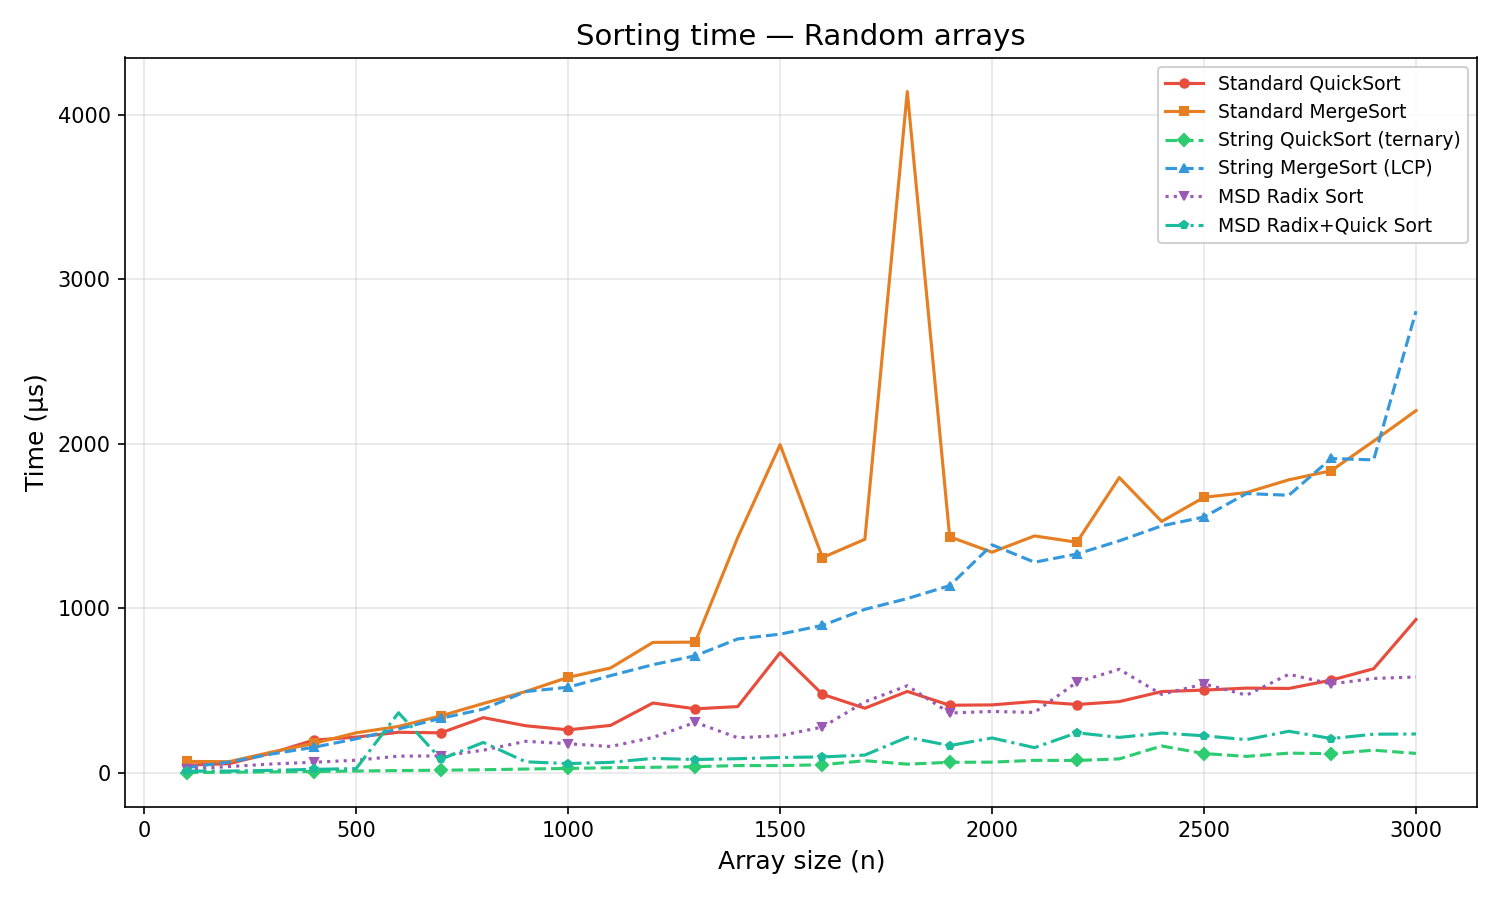
\includegraphics[width=\textwidth]{plots/time_random.png}
        \caption{Время выполнения}
    \end{subfigure}
    \hfill
    \begin{subfigure}[b]{0.48\textwidth}
        \centering
        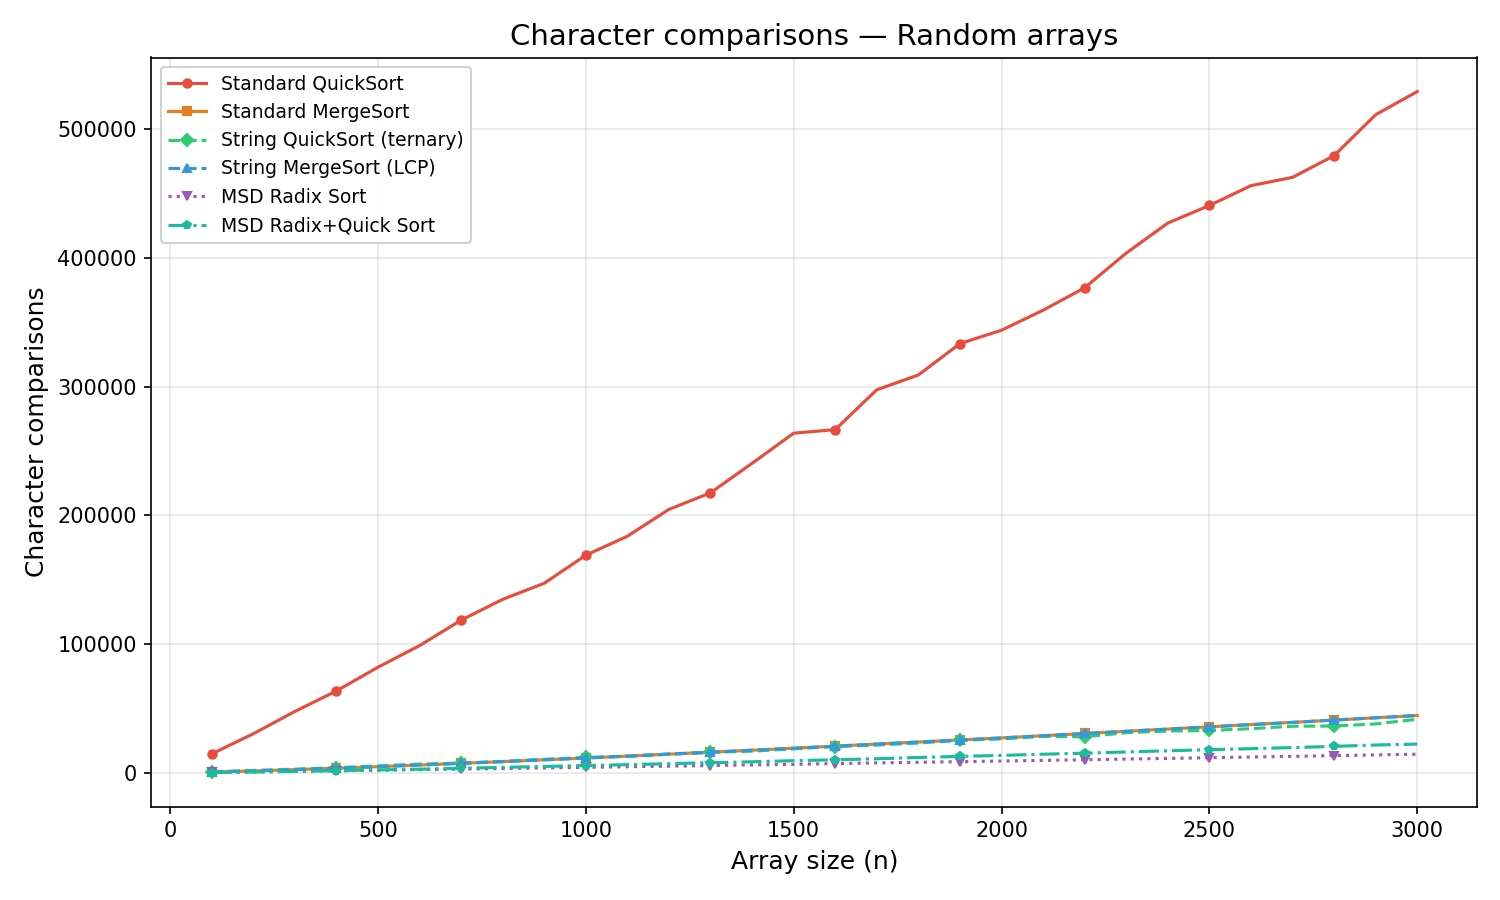
\includegraphics[width=\textwidth]{plots/comps_random.png}
        \caption{Количество посимвольных сравнений}
    \end{subfigure}
    \caption{Случайные массивы (random)}
\end{figure}

\subsection{Обратно отсортированные массивы}

\begin{figure}[H]
    \centering
    \begin{subfigure}[b]{0.48\textwidth}
        \centering
        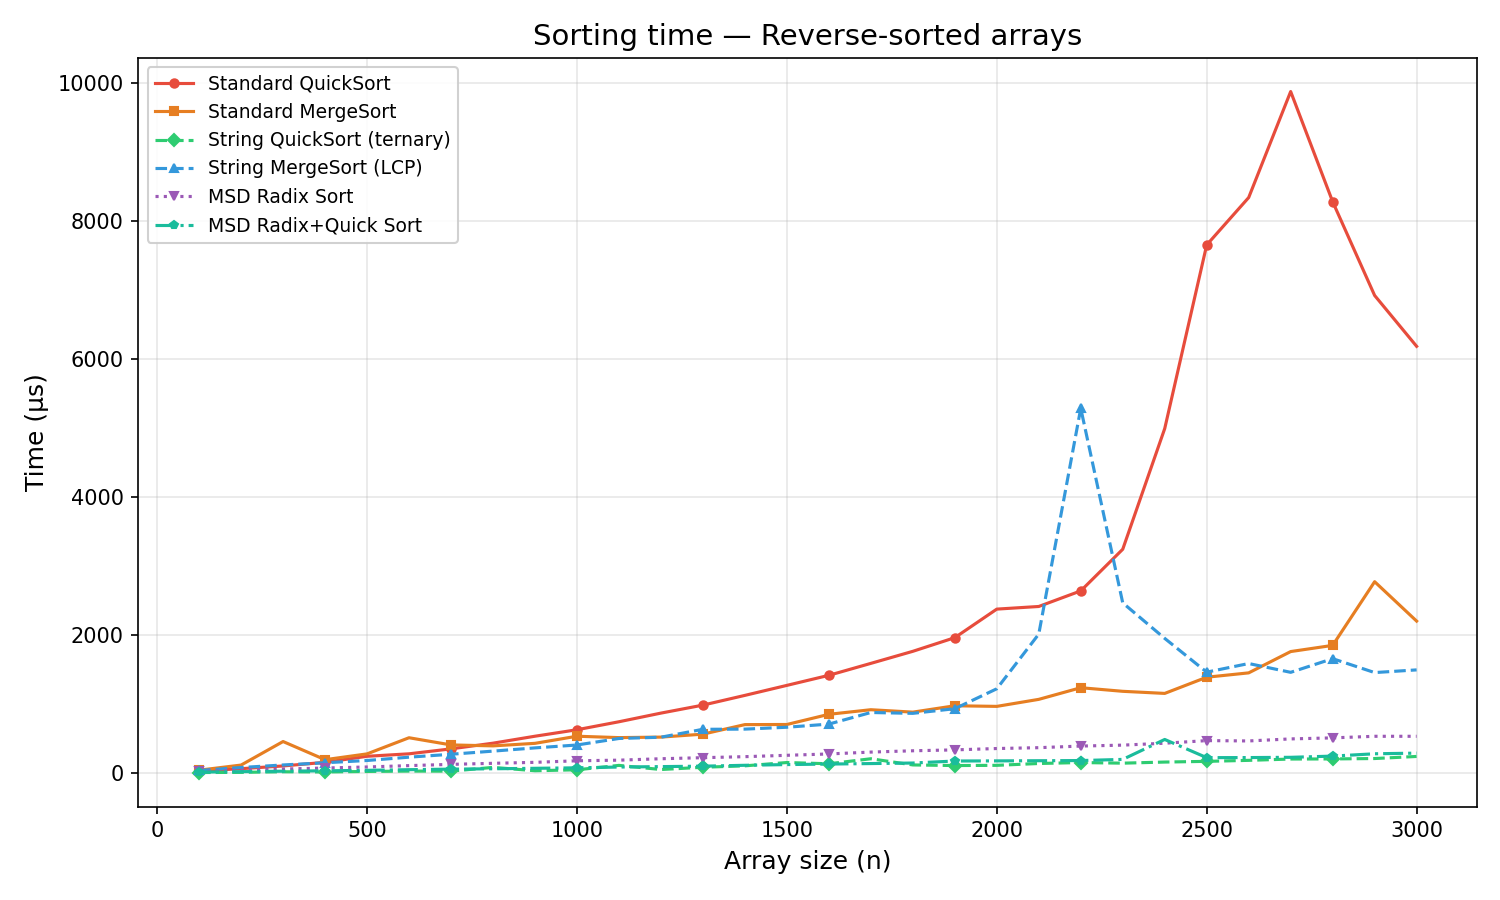
\includegraphics[width=\textwidth]{plots/time_reverse_sorted.png}
        \caption{Время выполнения}
    \end{subfigure}
    \hfill
    \begin{subfigure}[b]{0.48\textwidth}
        \centering
        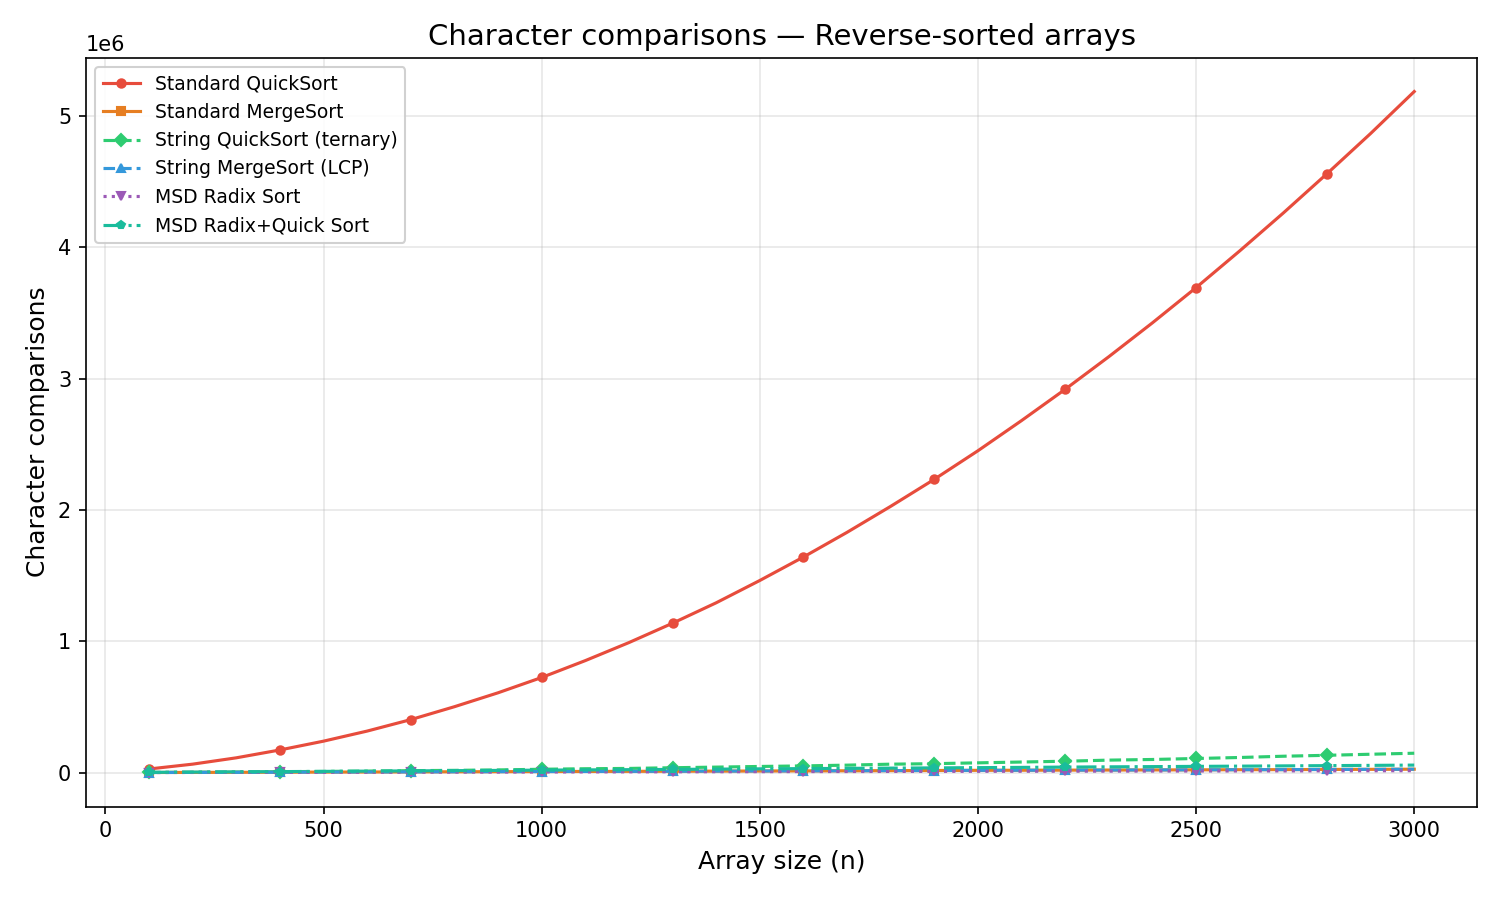
\includegraphics[width=\textwidth]{plots/comps_reverse_sorted.png}
        \caption{Количество посимвольных сравнений}
    \end{subfigure}
    \caption{Обратно отсортированные массивы (reverse sorted)}
\end{figure}

\subsection{Почти отсортированные массивы}

\begin{figure}[H]
    \centering
    \begin{subfigure}[b]{0.48\textwidth}
        \centering
        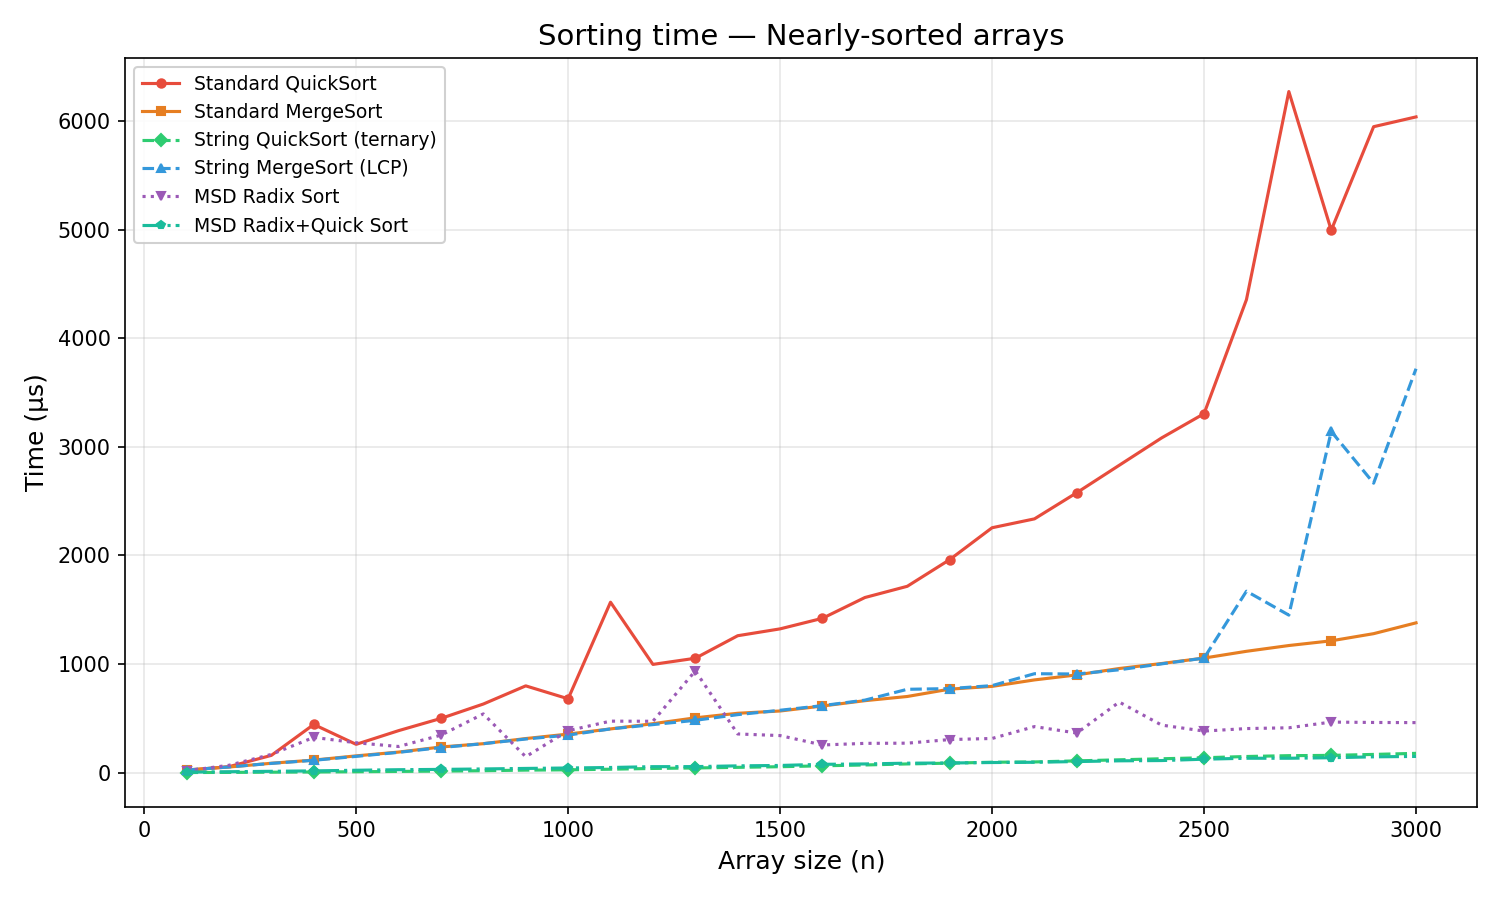
\includegraphics[width=\textwidth]{plots/time_nearly_sorted.png}
        \caption{Время выполнения}
    \end{subfigure}
    \hfill
    \begin{subfigure}[b]{0.48\textwidth}
        \centering
        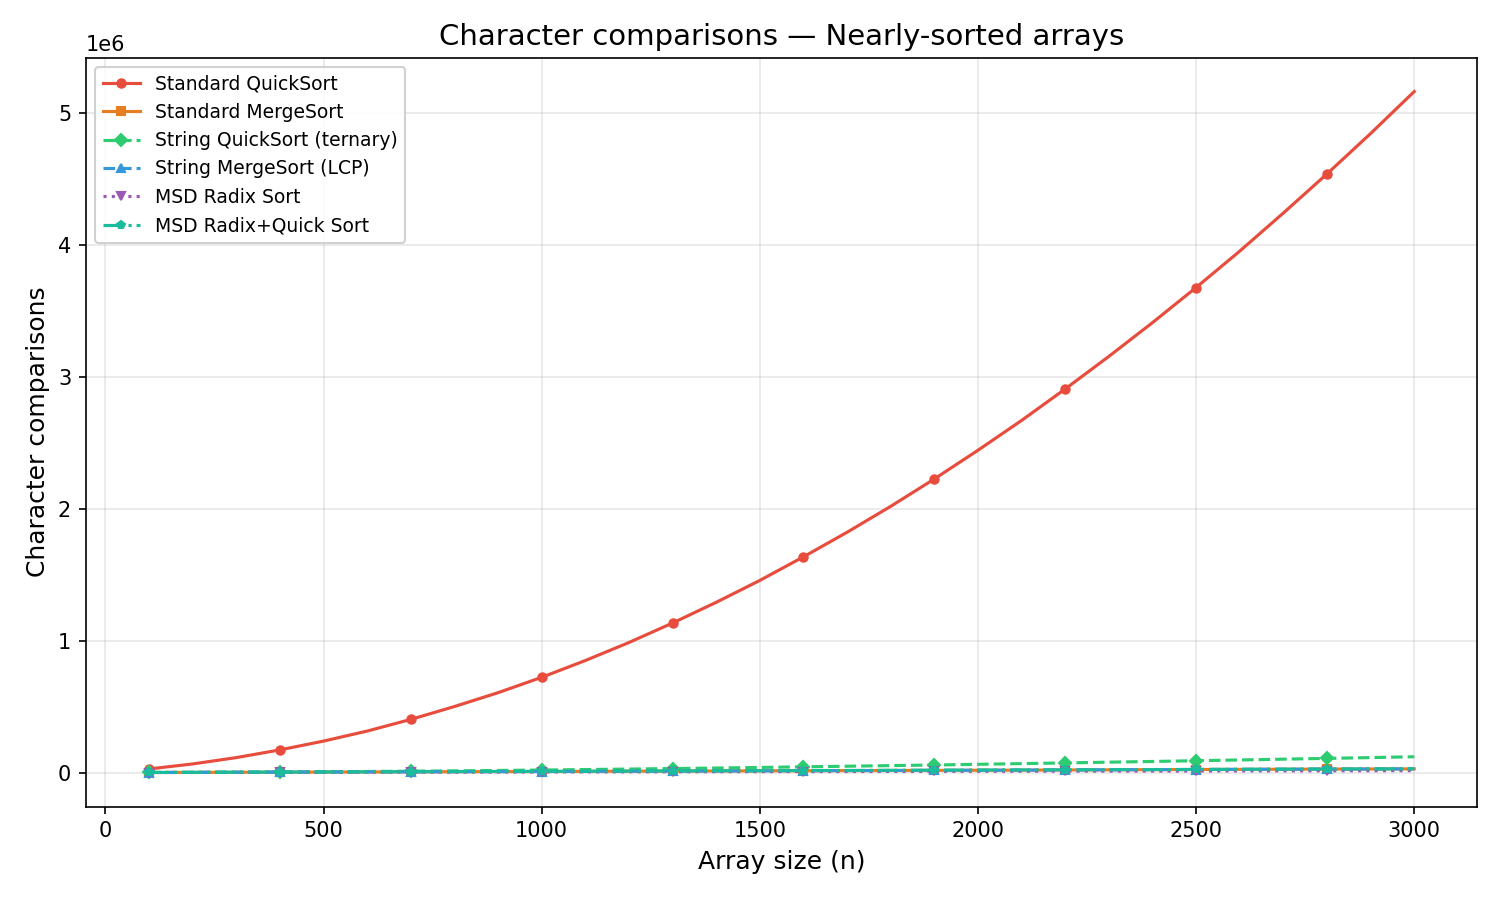
\includegraphics[width=\textwidth]{plots/comps_nearly_sorted.png}
        \caption{Количество посимвольных сравнений}
    \end{subfigure}
    \caption{Почти отсортированные массивы (nearly sorted)}
\end{figure}

\subsection{Массивы с общим префиксом}

\begin{figure}[H]
    \centering
    \begin{subfigure}[b]{0.48\textwidth}
        \centering
        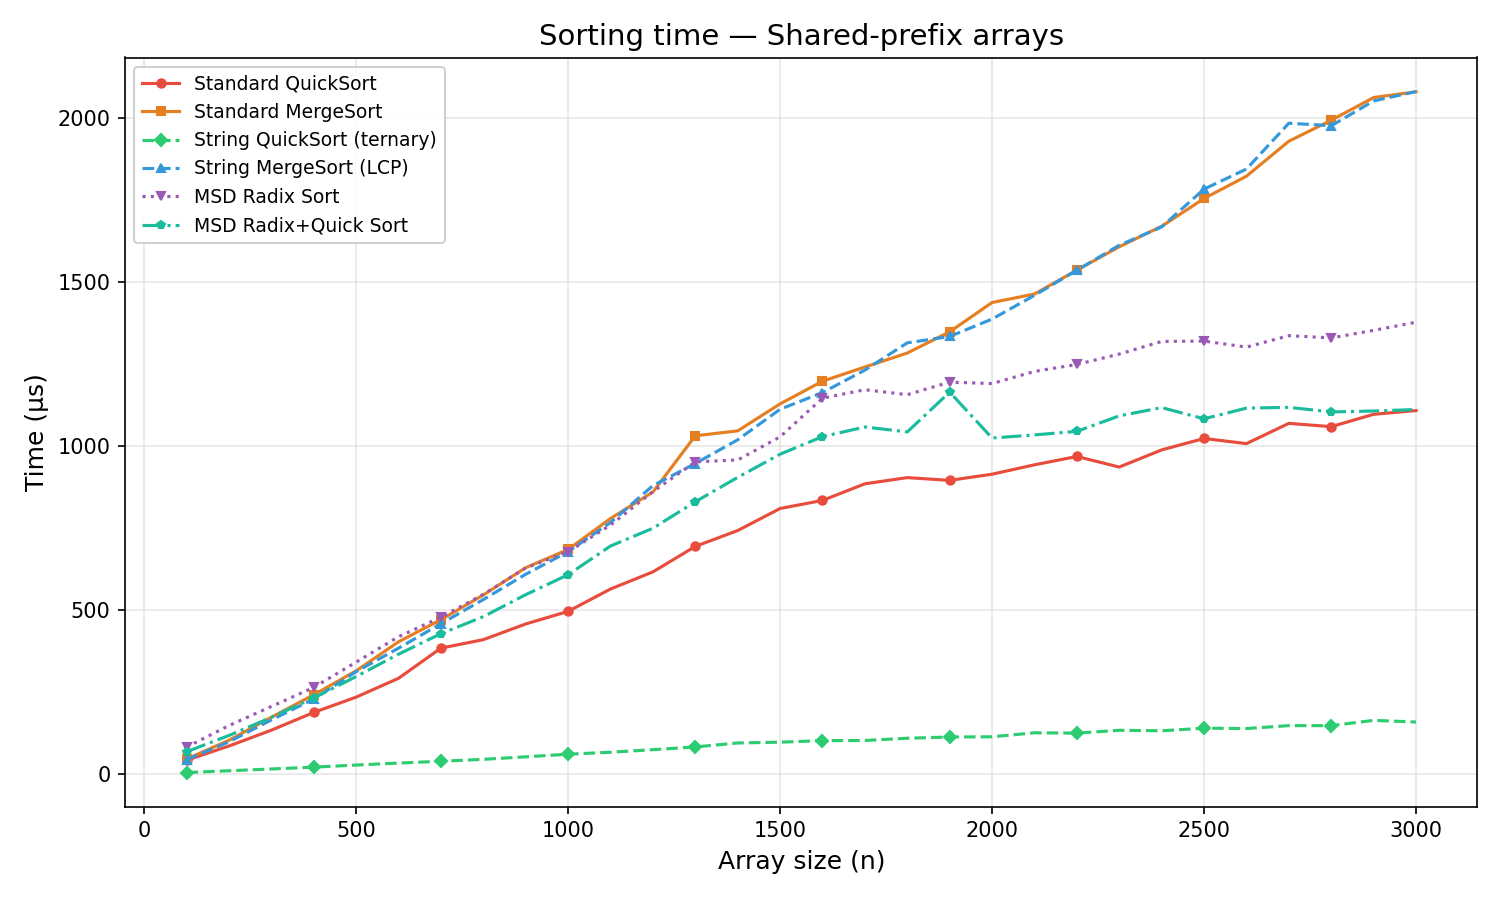
\includegraphics[width=\textwidth]{plots/time_shared_prefix.png}
        \caption{Время выполнения}
    \end{subfigure}
    \hfill
    \begin{subfigure}[b]{0.48\textwidth}
        \centering
        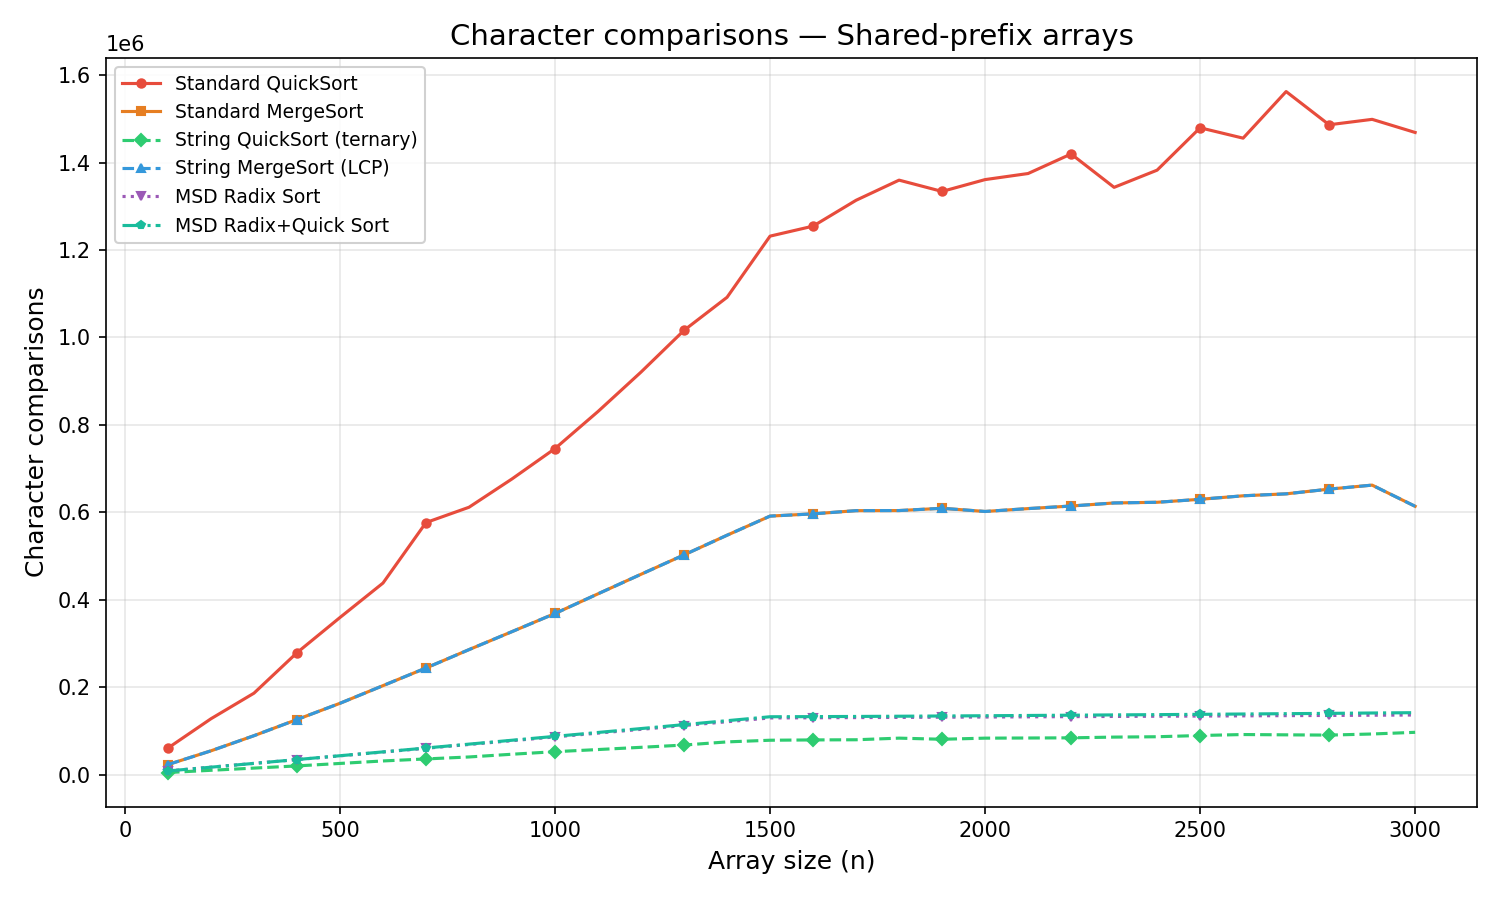
\includegraphics[width=\textwidth]{plots/comps_shared_prefix.png}
        \caption{Количество посимвольных сравнений}
    \end{subfigure}
    \caption{Массивы с общим префиксом (shared prefix)}
\end{figure}

\subsection{Сводный график (n = 3000)}

\begin{figure}[H]
    \centering
    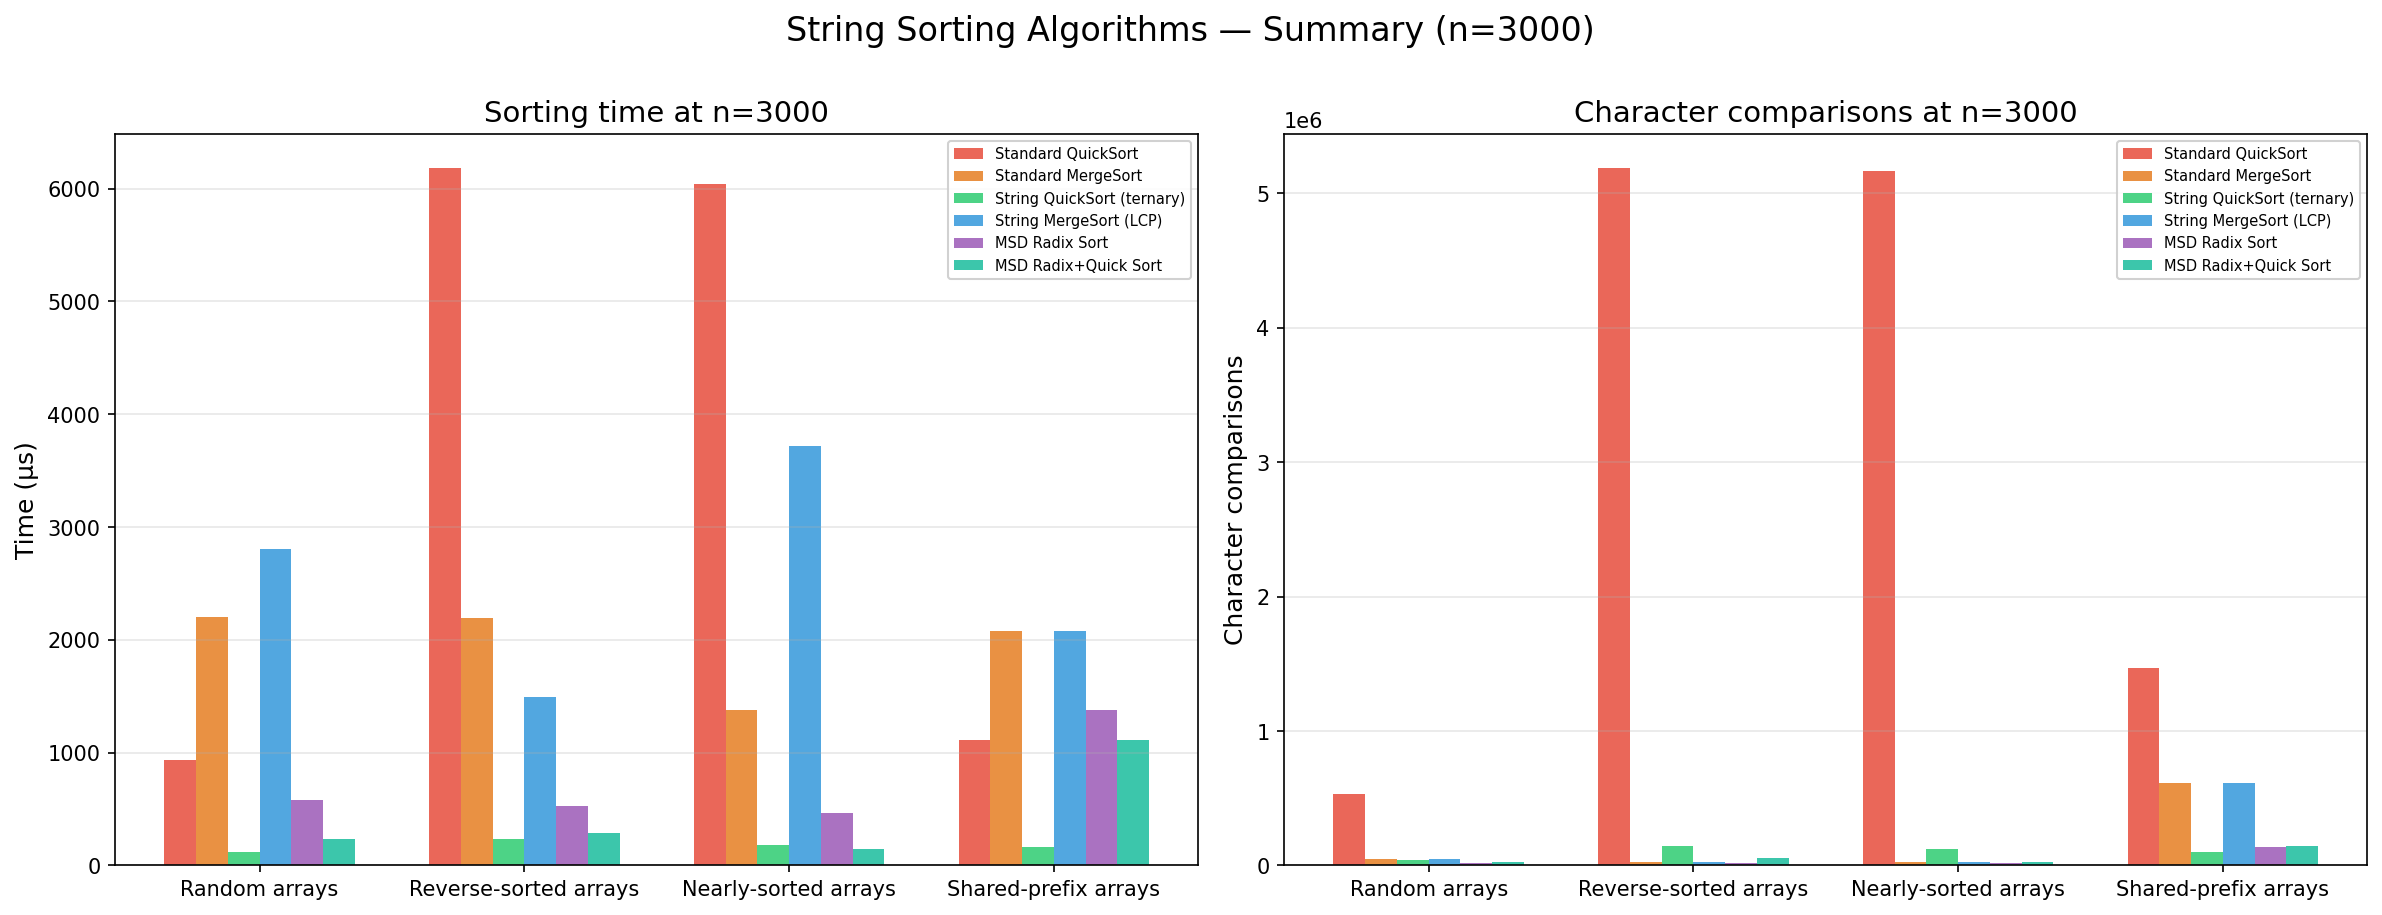
\includegraphics[width=\textwidth]{plots/summary.png}
    \caption{Сравнение всех алгоритмов при n = 3000}
\end{figure}

% ─── 4. Comparative analysis ─────────────────────────────────────────────────

\section{Сравнительный анализ}

\subsection{Стандартный QuickSort: деградация на упорядоченных данных}

Стандартный QuickSort с выбором первого элемента в качестве опорного демонстрирует катастрофическую деградацию на обратно отсортированных и почти отсортированных массивах. При $n = 3000$ число посимвольных сравнений достигает 5.2 млн, что более чем в 100 раз превышает показатели стандартного MergeSort (26\,000). Это классическое проявление worst-case поведения $O(n^2)$ при несбалансированном разбиении: на обратно отсортированном массиве опорный элемент (первый) всегда является наименьшим, что приводит к рекурсивному разбиению размера $n-1$ и $0$.

Стандартный MergeSort, напротив, сохраняет стабильную производительность: $\approx 26\,000$--$44\,000$ сравнений на всех типах данных, что соответствует теоретической оценке $O(n \log n)$ сравнений строк.

\subsection{String QuickSort: лидер по времени}

Тернарный String QuickSort является безоговорочным лидером по времени выполнения на всех четырёх типах тестовых данных. На случайных массивах размера 3000 он выполняется за 118~мкс, что в 8 раз быстрее стандартного QuickSort (932~мкс) и в 5 раз быстрее MSD Radix Sort (583~мкс).

Причина эффективности — в тернарном разбиении: строки с одинаковым символом на позиции~$d$ группируются вместе, и рекурсивная обработка средней части продолжается с позиции $d+1$, не пересравнивая уже совпавшие префиксы. Теоретическая сложность в среднем: $O(n \cdot L)$, где $L$ — средняя длина строки. Каждый символ в среднем просматривается константное число раз.

\subsection{MSD Radix Sort: минимальное число сравнений}

MSD Radix Sort демонстрирует наименьшее количество посимвольных сравнений среди всех алгоритмов (14\,500 на случайных массивах при $n=3000$), что соответствует теоретической оценке $O(n \cdot L)$. Однако по времени выполнения он уступает String QuickSort из-за накладных расходов: выделение массива счётчиков размера $R+2$, три прохода по подмассиву (подсчёт, копирование в aux, копирование обратно), рекурсивные вызовы для каждой из $R$ корзин.

\subsection{MSD Radix + Quick Sort: эффективный гибрид}

Гибридный алгоритм (переключение на String QuickSort при размере подмассива $< 74$) показывает хороший баланс: на случайных массивах — 236~мкс и 22\,000 сравнений, на почти отсортированных — 150~мкс и 29\,000 сравнений. Переключение на String QuickSort для малых подмассивов позволяет избежать накладных расходов count sort на глубоких уровнях рекурсии, где большинство корзин пусты.

\subsection{Влияние общего префикса}

Массивы с общим префиксом наиболее ярко демонстрируют преимущество адаптированных алгоритмов. Стандартный MergeSort делает 614\,000 посимвольных сравнений, тогда как String QuickSort — лишь 97\,000 (в 6.3 раза меньше). Причина в том, что стандартное сравнение строк каждый раз заново проходит общий префикс, в то время как String QuickSort, однажды обнаружив совпадение символов на позиции~$d$, переходит к позиции $d+1$ внутри сгруппированного блока равных строк.

Стандартный QuickSort на shared-prefix данных также страдает: 1.47 млн сравнений против 97\,000 у String QuickSort (в 15 раз хуже).

\subsection{Сравнение с теоретическими оценками}

\begin{table}[H]
\centering
\begin{tabular}{lcc}
\toprule
\textbf{Алгоритм} & \textbf{Теоретическая сложность} & \textbf{Подтверждено} \\
\midrule
Standard QuickSort  & $O(n \cdot L \cdot \log n)$ / $O(n^2 \cdot L)$ worst & Да \\
Standard MergeSort  & $O(n \cdot L \cdot \log n)$                            & Да \\
String QuickSort    & $O(n \cdot L)$ в среднем                               & Да \\
String MergeSort    & $O(n \cdot L \cdot \log n)$                            & Да \\
MSD Radix Sort      & $O(n \cdot L)$                                          & Да (по сравнениям) \\
MSD Radix + Quick   & $O(n \cdot L)$                                          & Да \\
\bottomrule
\end{tabular}
\caption{Теоретические оценки и их эмпирическое подтверждение}
\end{table}

Эмпирические данные согласуются с теоретическими оценками. Характер роста числа сравнений в зависимости от $n$ на графиках соответствует ожидаемому: линейный рост для MSD Radix и String QuickSort, $n \log n$ для MergeSort-вариантов, квадратичный для стандартного QuickSort на <<плохих>> данных.

% ─── Conclusion ──────────────────────────────────────────────────────────────

\section*{Заключение}

Проведён сравнительный эмпирический анализ шести алгоритмов сортировки строк на четырёх типах тестовых данных. Адаптированные строковые алгоритмы демонстрируют существенное преимущество над стандартными как по времени выполнения, так и по числу посимвольных сравнений. Тернарный String QuickSort является наилучшим выбором для большинства практических сценариев. MSD Radix Sort с переключением на String QuickSort представляет собой хороший компромисс между эффективностью по числу сравнений и временем выполнения.

% ─── Appendix: code listings ─────────────────────────────────────────────────

\appendix
\section{Листинги кода}

\subsection{string\_generator.h}

\lstinputlisting[language=C++]{string_generator.h}

\subsection{sort\_algorithms.h}

\lstinputlisting[language=C++]{sort_algorithms.h}

\subsection{string\_sort\_tester.h}

\lstinputlisting[language=C++]{string_sort_tester.h}

\end{document}
